%\documentclass{standalone}
%\documentclass[a4paper,class=article,border=0pt]{standalone}
\documentclass[tikz,margin=0.5pt]{standalone}
\usepackage{tikz}
\usepackage{pdftricks}
\begin{psinputs}
  \usepackage{pstricks}
  \usepackage{pst-node}
\end{psinputs}
%\documentclass{article}
%\documentclass[margin=3pt,pdftricks]{standalone}
%\begin{psinputs}
  %\usepackage{pstricks}
  %\usepackage{pst-node}
%\end{psinputs}
\usepackage{pgfplots}
\usepackage{xparse}
\usepackage{graphicx}
\usetikzlibrary{shapes,arrows,positioning}
\input{symbols-feyn}

\usetikzlibrary{positioning,arrows,patterns}
\usetikzlibrary{decorations.markings}
\usetikzlibrary{decorations.pathreplacing}
\usetikzlibrary{calc}

\tikzset{
  %photon/.style={decorate, decoration={snake,amplitude=5}, draw=black},
  photon/.style={decorate, decoration={snake}, draw=black},
  photonloop/.style={decorate, decoration={snake,segment length=8.3}, draw=black},
  higgs/.style={decorate, dashed, draw=black},
  fermion/.style={draw=black, postaction={decorate},
    decoration={markings,mark=at position .55 with {\arrow{>}}}},
  antifermion/.style={draw=black, postaction={decorate},
    decoration={markings,mark=at position .55 with {\arrow{<}}}},
  vertex/.style={draw,shape=circle,fill=black,minimum size=3pt,inner sep=0pt},
  svertex/.style={draw,shape=circle,fill=black,minimum size=0.75pt,inner sep=0pt},
}

%\NewDocumentCommand\semiloop{O{black}mmmO{}O{above}}
\NewDocumentCommand\semiloop{O{black}mmmmm}
{%
  %\draw[#1] let \p1 = ($(#3)-(#2)$) in (#3) arc
  %(#4:({#4+180}):({0.5*veclen(\x1,\y1)})node[midway, #6] {#5};)
  \draw[#1]
    let \p1 = (#2),
        \n1 = {(#3)},
        \n2 = {(#4)},
        \n3 = {(#5)}
        %\n2 = #4
        %\n3 = (#5)
        %\n1 = {0.5*veclen(\x1,\y1)}
    in (#2) #6 arc (\n3:\n2:\n1);
    %(#4:({180}):({#3})node[midway] {};)
  %(#4:({#4+180}):({0.5*veclen(\x1,\y1)})node[midway, #6] {#5};)
    %(45:({180}):({0.5*veclen(\x1,\y1)})node[midway, #6] {#5};)
    %(45:({180}):({0.5*veclen(\x1,\y1)})node[midway] {};)
      %(#2) arc (45:90:(\n1))
      %(#3) circle (\n1);
    %in (#3) arc
  %(#4:({#4+180}):({0.5*veclen(\x1,\y1)})node[midway, #6] {#5};)
}






% Flowchart
\tikzstyle{startstop} = [rectangle, rounded corners, minimum width=3cm, minimum height=1cm,text centered, draw=black, fill=red!30]
\tikzstyle{io} = [trapezium, trapezium left angle=70, trapezium right angle=110,
  minimum width=3cm, minimum height=1cm, text centered, draw=black,
fill=blue!30]
\tikzstyle{process} = [rectangle, minimum width=3cm, minimum height=1cm, text
centered, draw=black, fill=orange!30]
\tikzstyle{decision} = [diamond, minimum width=3cm, minimum height=1cm, text
centered, draw=black, fill=green!30]
\tikzstyle{arrow} = [thick,->,>=stealth]




\begin{document}
\begin{tikzpicture}[node distance=1cm and 1cm,line width=1.1pt]
  \coordinate[] (i1);
  \coordinate[below=1 of i1,label=left:\bquarkbar] (i2);
  \coordinate[below=2 of i1] (i3);
  \coordinate[below=3 of i1,label=left:\uquark] (i4);
  \coordinate[below=4 of i1] (i5);
  \coordinate[vertex,right=1 of i3,label=below right:$V_{ub}^*$] (v1);
  \coordinate[vertex,right=1.4 of v1,label=below left:$V_{cs}^{}$] (v2);
  \coordinate[vertex,right=1 of v2] (v3);
  \coordinate[right=1 of v3] (o3);
  \coordinate[above=2 of o3,label=right:\cquarkbar] (o1);
  \coordinate[above=1 of o3,label=right:\squark] (o2);
  \coordinate[below=1 of o3,label=right:\squarkbar] (o4);
  \coordinate[below=2 of o3,label=right:\squark] (o5);
  \draw[fermion] (i2) -- (v1);
  \draw[fermion] (v1) -- (i4);
  \draw[fermion] (o1) -- (v2);
  \draw[fermion] (v2) -- (o5);
  \draw[fermion] (o4) -- (v3);
  \draw[fermion] (v3) -- (o2);
  \draw[photon] (v1) -- (v2) node[midway,above=0.1] {$W^+$};
  \coordinate[above left=0.5 of i2] (bi1);
  \coordinate[below left=0.5 of i4] (bi2);
  \coordinate[above right=0.5 of o1] (bo1);
  \coordinate[below right=0.5 of o2] (bo2);
  \coordinate[above right=0.5 of o4] (bo3);
  \coordinate[below right=0.5 of o5] (bo4);
  \draw [decorate,decoration={brace,amplitude=10pt},xshift=4pt,yshift=0pt]
  (bi2) -- (bi1) node [black,midway,xshift=-0.8cm] {$\Bp$};
  \draw [decorate,decoration={brace,amplitude=10pt},xshift=4pt,yshift=0pt]
  (bo1) -- (bo2) node [black,midway,xshift=0.7cm] {$\Dsp$};
  \draw [decorate,decoration={brace,amplitude=10pt},xshift=4pt,yshift=0pt]
  (bo3) -- (bo4) node [black,midway,xshift=0.6cm] {$\phi$};
\end{tikzpicture}

%\newpage
%\pagebreak


\begin{tikzpicture}[node distance=1cm and 1cm,line width=1.1pt]
  \coordinate[] (i1);
  \coordinate[below=1 of i1,label=left:\bquarkbar] (i2);
  \coordinate[below=2 of i1] (i3);
  \coordinate[below=3 of i1,label=left:\uquark] (i4);
  \coordinate[below=4 of i1] (i5);
  \coordinate[vertex,right=1 of i3] (v1);
  \coordinate[vertex,right=1.4 of v1] (v2);
  \coordinate[vertex,right=1 of v2] (v3);
  \coordinate[right=1 of v3] (o3);
  \coordinate[above=2 of o3,label=right:\cquarkbar] (o1);
  \coordinate[above=1 of o3,label=right:\squark] (o2);
  \coordinate[below=1 of o3,label=right:\squarkbar] (o4);
  \coordinate[below=2 of o3,label=right:\squark] (o5);
  \draw[fermion] (i2) -- (v1);
  \draw[fermion] (v1) -- (i4);
  \draw[fermion] (o1) -- (v2);
  \draw[fermion] (v2) -- (o5);
  \draw[fermion] (o4) -- (v3);
  \draw[fermion] (v3) -- (o2);
  \draw[higgs] (v1) -- (v2) node[midway,above=0.1] {$H^+$};
  \coordinate[above left=0.4 of i2] (bi1);
  \coordinate[below left=0.4 of i4] (bi2);
  \coordinate[above right=0.4 of o1] (bo1);
  \coordinate[below right=0.4 of o2] (bo2);
  \coordinate[above right=0.4 of o4] (bo3);
  \coordinate[below right=0.4 of o5] (bo4);
  \draw [decorate,decoration={brace,amplitude=10pt},xshift=4pt,yshift=0pt]
  (bi2) -- (bi1) node [black,midway,xshift=-0.7cm] {$\Bp$};
  \draw [decorate,decoration={brace,amplitude=10pt},xshift=4pt,yshift=0pt]
  (bo1) -- (bo2) node [black,midway,xshift=0.7cm] {$\Dsp$};
  \draw [decorate,decoration={brace,amplitude=10pt},xshift=4pt,yshift=0pt]
  (bo3) -- (bo4) node [black,midway,xshift=0.6cm] {$\phi$};
\end{tikzpicture}


%\begin{tikzpicture}[node distance=1cm and 1cm,line width=1.1pt]
  %%[line width=1.5 pt, scale=1.3]
  %\coordinate[label=left:\bquarkbar] (i1);
  %\coordinate[label=left:\uquark,below=5 of i1] (i2);
  %\coordinate[label=above left:$V_{tb}$,vertex,right=1.5 of i1] (v1);
  %\coordinate[label=above right:$V_{ts}$,vertex,right=2 of v1] (v2);
  %\coordinate[right=0.8 of v2] (d2);
  %\coordinate[left=0.3 of v2] (d3);
  %\coordinate[vertex,below=1.5 of d2] (v3);
  %\coordinate[vertex,below=3.5 of d2] (v4);
  %\coordinate[vertex,above=0.7 of d3] (v5);
  %\coordinate[vertex,above=1.5 of d2] (v6);
  %\coordinate[label=right:\squarkbar,right=1.8 of v2] (o1);
  %\coordinate[label=right:\uquark,below=1 of o1] (o2);
  %\coordinate[label=right:\uquarkbar,below=2 of o1] (o3);
  %\coordinate[label=right:\dquark,below=3 of o1] (o4);
  %\coordinate[label=right:\dquarkbar,below=4 of o1] (o5);
  %\coordinate[label=right:\uquark,below=5 of o1] (o6);
  %\coordinate[label=right:\mun,above=1 of o1] (o7);
  %\coordinate[label=right:\mup,above=2 of o1] (o8);
  %\draw[antifermion] (v1) arc (180:0:1.05) ++(-1.3,1.3) node[left] {\tquarkbar};
  %\draw[photonloop] (v2) arc (0:-180:1.05) ++(1.5,-0.7) node[left] {$W^+$};
  %\draw[antifermion] (i1) -- (v1);
  %\draw[fermion] (i2) -- (o6);
  %\draw[antifermion] (v2) -- (o1);
  %\draw[fermion] (v3) -- (o2);
  %\draw[antifermion] (v3) -- (o3);
  %\draw[fermion] (v4) -- (o4);
  %\draw[antifermion] (v4) -- (o5);
  %\draw[photon] (v6) -- (v5);
  %\draw[fermion] (v6) -- (o7);
  %\draw[antifermion] (v6) -- (o8);
  %\coordinate[above left=0.5 of i1] (bi1);
  %\coordinate[below left=0.5 of i2] (bi2);
  %\coordinate[above right=0.5 of o1] (bo1);
  %\coordinate[below right=0.5 of o2] (bo2);
  %\coordinate[above right=0.5 of o3] (bo3);
  %\coordinate[below right=0.5 of o4] (bo4);
  %\coordinate[above right=0.5 of o5] (bo5);
  %\coordinate[below right=0.5 of o6] (bo6);
  %\draw [decorate,decoration={brace,amplitude=10pt},xshift=4pt,yshift=0pt]
  %(bi2) -- (bi1) node [black,midway,xshift=-0.7cm] {$B^+$};
  %\draw [decorate,decoration={brace,amplitude=10pt},xshift=4pt,yshift=0pt]
  %(bo1) -- (bo2) node [black,midway,xshift=0.7cm] {$K^+$};
  %\draw [decorate,decoration={brace,amplitude=10pt},xshift=4pt,yshift=0pt]
  %(bo3) -- (bo4) node [black,midway,xshift=0.7cm] {$\pi^-$};
  %\draw [decorate,decoration={brace,amplitude=10pt},xshift=4pt,yshift=0pt]
  %(bo5) -- (bo6) node [black,midway,xshift=0.7cm] {$\pi^+$};
%\end{tikzpicture}


%\begin{tikzpicture}[node distance=1cm and 1cm,line width=1.1pt]
  %\coordinate[label=left:\bquarkbar] (i1);
  %\coordinate[label=left:\uquark,below=3.0 of i1] (i2);
  %\coordinate[label=above left:$V_{tb}$,vertex,right=1.5 of i1] (v1);
  %\coordinate[label=above right:$V_{ts}$,vertex,right=2 of v1] (v2);
  %\coordinate[right=0.8 of v2] (d2);
  %\coordinate[left=0.3 of v2] (d3);
  %\coordinate[vertex,below=1.5 of d2] (v3);
  %\coordinate[vertex,above=0.7 of d3] (v5);
  %\coordinate[vertex,above=1.5 of d2] (v6);
  %\coordinate[label=right:\squarkbar,right=1.8 of v2] (o1);
  %\coordinate[label=right:\squark,below=1 of o1] (o2);
  %\coordinate[label=right:\squarkbar,below=2 of o1] (o3);
  %\coordinate[label=right:\uquark,below=3 of o1] (o4);
  %\coordinate[label=right:\mun,above=1 of o1] (o7);
  %\coordinate[label=right:\mup,above=2 of o1] (o8);
  %\draw[antifermion] (v1) arc (180:0:1.05) ++(-1.3,1.3) node[left] {\tquarkbar};
  %\draw[photonloop] (v2) arc (0:-180:1.05) ++(1.5,-0.7) node[left] {$W^+$};
  %\draw[antifermion] (i1) -- (v1);
  %\draw[fermion] (i2) -- (o4);
  %\draw[antifermion] (v2) -- (o1);
  %\draw[fermion] (v3) -- (o2);
  %\draw[antifermion] (v3) -- (o3);
  %\draw[photon] (v6) -- (v5);
  %\draw[fermion] (v6) -- (o7);
  %\draw[antifermion] (v6) -- (o8);
  %\coordinate[above left=0.5 of i1] (bi1);
  %\coordinate[below left=0.5 of i2] (bi2);
  %\coordinate[above right=0.5 of o1] (bo1);
  %\coordinate[below right=0.5 of o2] (bo2);
  %\coordinate[above right=0.5 of o3] (bo3);
  %\coordinate[below right=0.5 of o4] (bo4);
  %\draw [decorate,decoration={brace,amplitude=10pt},xshift=4pt,yshift=0pt]
  %(bi2) -- (bi1) node [black,midway,xshift=-0.7cm] {$B^+$};
  %\draw [decorate,decoration={brace,amplitude=10pt},xshift=4pt,yshift=0pt]
  %(bo1) -- (bo2) node [black,midway,xshift=0.6cm] {$\phi$};
  %\draw [decorate,decoration={brace,amplitude=10pt},xshift=4pt,yshift=0pt]
  %(bo3) -- (bo4) node [black,midway,xshift=0.7cm] {$K^+$};
%\end{tikzpicture}


\begin{tikzpicture}[node distance=1cm and 1cm,line width=1.1pt]
  %[line width=1.5 pt, scale=1.3]
  \coordinate[label=left:\bquarkbar] (i1);
  \coordinate[label=left:\uquark,below=5 of i1] (i2);
  \coordinate[label=above left:$V_{tb}$,vertex,right=1.5 of i1] (v1);
  \coordinate[label=above right:$V_{ts}$,vertex,right=1.6 of v1] (v2);
  \coordinate[right=0.6 of v2] (d2);
  \coordinate[left=0.3 of v2] (d3);
  \coordinate[vertex,below=1.5 of d2] (v3);
  \coordinate[vertex,below=3.5 of d2] (v4);
  \coordinate[vertex,above=0.6 of d3] (v5);
  \coordinate[vertex,above=1.5 of d2] (v6);
  \coordinate[label=right:\squarkbar,right=1.6 of v2] (o1);
  \coordinate[label=right:\uquark,below=1 of o1] (o2);
  \coordinate[label=right:\uquarkbar,below=2 of o1] (o3);
  \coordinate[label=right:\dquark,below=3 of o1] (o4);
  \coordinate[label=right:\dquarkbar,below=4 of o1] (o5);
  \coordinate[label=right:\uquark,below=5 of o1] (o6);
  \coordinate[label=right:\mun,above=1 of o1] (o7);
  \coordinate[label=right:\mup,above=2 of o1] (o8);
  \draw[antifermion] (v1) arc (180:0:0.85) ++(-1.1,1.0) node[left] {\tquarkbar};
  \draw[photonloop] (v2) arc (0:-180:0.85) ++(1.4,-0.55) node[left] {$W^+$};
  \draw[antifermion] (i1) -- (v1);
  \draw[fermion] (i2) -- (o6);
  \draw[antifermion] (v2) -- (o1);
  \draw[fermion] (v3) -- (o2);
  \draw[antifermion] (v3) -- (o3);
  \draw[fermion] (v4) -- (o4);
  \draw[antifermion] (v4) -- (o5);
  \draw[photon] (v6) -- (v5);
  \draw[fermion] (v6) -- (o7);
  \draw[antifermion] (v6) -- (o8);
  \coordinate[above left=0.5 of i1] (bi1);
  \coordinate[below left=0.5 of i2] (bi2);
  \coordinate[above right=0.5 of o1] (bo1);
  \coordinate[below right=0.5 of o2] (bo2);
  \coordinate[above right=0.5 of o3] (bo3);
  \coordinate[below right=0.5 of o4] (bo4);
  \coordinate[above right=0.5 of o5] (bo5);
  \coordinate[below right=0.5 of o6] (bo6);
  \draw [decorate,decoration={brace,amplitude=10pt},xshift=4pt,yshift=0pt]
  (bi2) -- (bi1) node [black,midway,xshift=-0.7cm] {$B^+$};
  \draw [decorate,decoration={brace,amplitude=10pt},xshift=4pt,yshift=0pt]
  (bo1) -- (bo2) node [black,midway,xshift=0.7cm] {$K^+$};
  \draw [decorate,decoration={brace,amplitude=10pt},xshift=4pt,yshift=0pt]
  (bo3) -- (bo4) node [black,midway,xshift=0.7cm] {$\pi^-$};
  \draw [decorate,decoration={brace,amplitude=10pt},xshift=4pt,yshift=0pt]
  (bo5) -- (bo6) node [black,midway,xshift=0.7cm] {$\pi^+$};
\end{tikzpicture}


\begin{tikzpicture}[node distance=1cm and 1cm,line width=1.1pt]
  %[line width=1.5 pt, scale=1.3]
  \coordinate[label=left:\bquarkbar] (i1);
  \coordinate[label=left:\uquark,below=3 of i1] (i2);
  \coordinate[label=above left:$V_{tb}$,vertex,right=1.5 of i1] (v1);
  \coordinate[label=above right:$V_{ts}$,vertex,right=1.6 of v1] (v2);
  \coordinate[right=0.6 of v2] (d2);
  \coordinate[left=0.3 of v2] (d3);
  \coordinate[vertex,below=1.5 of d2] (v3);
  \coordinate[vertex,above=0.6 of d3] (v5);
  \coordinate[vertex,above=1.5 of d2] (v6);
  \coordinate[label=right:\squarkbar,right=1.6 of v2] (o1);
  \coordinate[label=right:\squark,below=1 of o1] (o2);
  \coordinate[label=right:\squarkbar,below=2 of o1] (o3);
  \coordinate[label=right:\uquark,below=3 of o1] (o4);
  \coordinate[label=right:\mun,above=1 of o1] (o7);
  \coordinate[label=right:\mup,above=2 of o1] (o8);
  \draw[antifermion] (v1) arc (180:0:0.85) ++(-1.1,1.0) node[left] {\tquarkbar};
  \draw[photonloop] (v2) arc (0:-180:0.85) ++(1.4,-0.55) node[left] {$W^+$};
  \draw[antifermion] (i1) -- (v1);
  \draw[fermion] (i2) -- (o4);
  \draw[antifermion] (v2) -- (o1);
  \draw[fermion] (v3) -- (o2);
  \draw[antifermion] (v3) -- (o3);
  \draw[photon] (v6) -- (v5);
  \draw[fermion] (v6) -- (o7);
  \draw[antifermion] (v6) -- (o8);
  \coordinate[above left=0.5 of i1] (bi1);
  \coordinate[below left=0.5 of i2] (bi2);
  \coordinate[above right=0.5 of o1] (bo1);
  \coordinate[below right=0.5 of o2] (bo2);
  \coordinate[above right=0.5 of o3] (bo3);
  \coordinate[below right=0.5 of o4] (bo4);
  \draw [decorate,decoration={brace,amplitude=10pt},xshift=4pt,yshift=0pt]
  (bi2) -- (bi1) node [black,midway,xshift=-0.7cm] {$B^+$};
  \draw [decorate,decoration={brace,amplitude=10pt},xshift=4pt,yshift=0pt]
  (bo1) -- (bo2) node [black,midway,xshift=0.6cm] {$\phi$};
  \draw [decorate,decoration={brace,amplitude=10pt},xshift=4pt,yshift=0pt]
  (bo3) -- (bo4) node [black,midway,xshift=0.7cm] {$K^+$};
\end{tikzpicture}


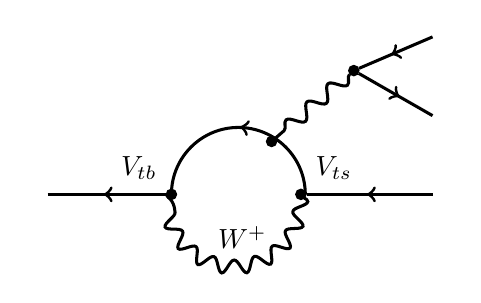
\begin{tikzpicture}[node distance=1cm and 1cm,line width=1.1pt]
  \coordinate[label=left:\bquarkbar] (i1);
  \coordinate[label=above left:$V_{tb}$,vertex,right=1.5 of i1] (v1);
  \coordinate[label=above right:$V_{ts}$,vertex,right=1.5 of v1] (v2);
  \coordinate[right=0.6 of v2] (d2);
  \coordinate[left=0.3 of v2] (d3);
  \coordinate[vertex,above=0.6 of d3] (v5);
  \coordinate[vertex,above=1.5 of d2] (v6);
  \coordinate[label=right:\squarkbar,right=1.6 of v2] (o1);
  \coordinate[label=right:\mun,above=1 of o1] (o7);
  \coordinate[label=right:\mup,above=2 of o1] (o8);
  \draw[antifermion] (v1) arc (180:0:0.85) ++(-1.1,1.0) node[left] {\tquarkbar};
  \draw[photonloop] (v2) arc (0:-180:0.85) ++(1.4,-0.55) node[left] {$W^+$};
  \draw[antifermion] (i1) -- (v1);
  \draw[antifermion] (v2) -- (o1);
  \draw[photon] (v6) -- (v5);
  \draw[fermion] (v6) -- (o7);
  \draw[antifermion] (v6) -- (o8);
\end{tikzpicture}


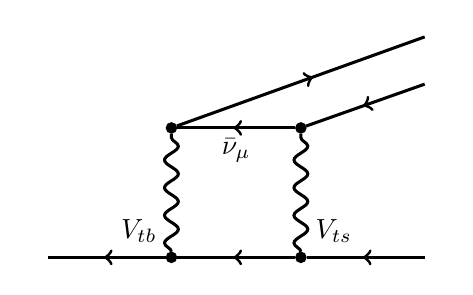
\begin{tikzpicture}[node distance=1cm and 1cm,line width=1.1pt]
  \coordinate[label=left:\bquarkbar] (i1);
  \coordinate[label=above left:$V_{tb}$,vertex,right=1.5 of i1] (v1);
  \coordinate[vertex,above=1.5 of v1] (v2);
  \coordinate[label=above right:$V_{ts}$,vertex,right=1.5 of v1] (v3);
  \coordinate[vertex,right=1.5 of v2] (v4);
  \coordinate[label=right:\squarkbar,right=1.5 of v3] (o1);
  \coordinate[label=right:\mup,above=2.2 of o1] (o2);
  \coordinate[label=right:\mun,above=2.8 of o1] (o3);
  \draw[antifermion] (i1) -- (v1);
  \draw[antifermion] (v1) -- (v3) node[midway,above] {$\tquarkbar$};
  \draw[antifermion] (v3) -- (o1);
  \draw[antifermion] (v2) -- (v4) node[midway,below] {$\bar{\nu}_\mu$};
  \draw[photon] (v1) -- (v2);
  \draw[photon] (v3) -- (v4);
  \draw[fermion] (v2) -- (o3);
  \draw[antifermion] (v4) -- (o2);
\end{tikzpicture}


\begin{tikzpicture}[node distance=1cm and 1cm,line width=1.1pt]
  %[line width=1.5 pt, scale=1.3]
  \coordinate[label=left:\bquarkbar] (i1);
  \coordinate[label=left:\dquark,below=3 of i1] (i2);
  \coordinate[label=above left:$V_{tb}$,vertex,right=1.5 of i1] (v1);
  \coordinate[label=above right:$V_{ts}$,vertex,right=1.6 of v1] (v2);
  \coordinate[right=0.6 of v2] (d2);
  \coordinate[left=0.3 of v2] (d3);
  %\coordinate[vertex,below=1.5 of d2] (v3);
  \coordinate[vertex,above=0.6 of d3] (v5);
  \coordinate[vertex,above=1.5 of d2] (v6);
  \coordinate[label=right:\squarkbar,right=1.6 of v2] (o1);
  %\coordinate[label=right:\squark,below=1 of o1] (o2);
  %\coordinate[label=right:\squarkbar,below=2 of o1] (o3);
  \coordinate[label=right:\dquark,below=3 of o1] (o2);
  \coordinate[label=right:\mun,above=1 of o1] (o7);
  \coordinate[label=right:\mup,above=2 of o1] (o8);
  \draw[antifermion] (v1) arc (180:0:0.85) ++(-1.1,1.0) node[left] {\tquarkbar};
  \draw[photonloop] (v2) arc (0:-180:0.85) ++(1.4,-0.55) node[left] {$W^+$};
  \draw[antifermion] (i1) -- (v1);
  \draw[fermion] (i2) -- (o2);
  \draw[antifermion] (v2) -- (o1);
  %\draw[fermion] (v3) -- (o2);
  %\draw[antifermion] (v3) -- (o3);
  \draw[higgs] (v6) -- (v5) node[midway,above left] {$\chi$};
  \draw[fermion] (v6) -- (o7);
  \draw[antifermion] (v6) -- (o8);
  \coordinate[above left=0.5 of i1] (bi1);
  \coordinate[below left=0.5 of i2] (bi2);
  \coordinate[above right=0.5 of o1] (bo1);
  \coordinate[below right=0.5 of o2] (bo2);
  %\coordinate[above right=0.5 of o3] (bo3);
  %\coordinate[below right=0.5 of o4] (bo4);
  \draw [decorate,decoration={brace,amplitude=10pt},xshift=4pt,yshift=0pt]
  (bi2) -- (bi1) node [black,midway,xshift=-0.7cm] {$B^0$};
  \draw [decorate,decoration={brace,amplitude=10pt},xshift=4pt,yshift=0pt]
  (bo1) -- (bo2) node [black,midway,xshift=0.7cm] {$\Kstarz$};
\end{tikzpicture}


%\begin{tikzpicture}[node distance=1cm and 1cm,line width=1.1pt]
  %%[line width=1.5 pt, scale=1.3]
  %\coordinate[vertex, label=left:\bquarkbar] (i0);
  %\coordinate[vertex, below=2.5 of i0, label=left:\dquark] (i1);
  %\coordinate[right=2 of i1] (d1);
  %\coordinate[right=2 of d1] (d2);
  %\coordinate[vertex, right=2 of d2, label=right:\dquark] (o3);
  %\coordinate[vertex, above=1 of o3, label=right:$\cquark/\uquark$] (o2);
  %\coordinate[vertex, above=2 of o3, label=right:\uquark] (o1);
  %\coordinate[vertex, above=3 of o3, label=right:\mun] (o0);
  %\coordinate[right=0.25 of o1] (d3);
  %\coordinate[right=0.25 of o3] (d4);
  %\coordinate[vertex, above=1.5 of d2, label=above:?$_2$] (v1);
  %\coordinate[vertex, above=2.5 of d1, label=above:?$_1$] (v0);
  %\draw[fermion] (v0) -- (i0);
  %\draw[fermion] (o0) -- (v0);
  %\draw[fermion] (v1) -- (o1);
  %\draw[fermion] (v1) -- (o2);
  %\draw[fermion] (i1) -- (o3);
  %\draw[higgs] (v0) -- (v1) node [midway,below left] {$+\tfrac43$};
  %\coordinate[above left=0.5 of i0] (bi0);
  %\coordinate[below left=0.5 of i1] (bi1);
  %\coordinate[above right=0.5 of d3] (bo0);
  %\coordinate[below right=0.5 of d4] (bo1);
  %\draw [decorate,decoration={brace,amplitude=10pt},xshift=4pt,yshift=0pt]
  %(bi1) -- (bi0) node [black,midway,xshift=-0.7cm] {$B^0$};
  %\draw [decorate,decoration={brace,amplitude=10pt},xshift=4pt,yshift=0pt]
  %(bo0) -- (bo1) node [black,midway,xshift=0.9cm] {$\Lc/p$};
%\end{tikzpicture}


%\begin{tikzpicture}[node distance=1cm and 1cm,line width=1.1pt]
\begin{tikzpicture} [line width=1.5 pt, scale=1.3]
  %[line/.style={-,shorten >=0.4cm,shorten <=0.4cm},thick]
  %%%%%%%
  % (rho,eta) = (0.131,0.345) * 5 = (0.655,1.725)
  % gamma = 68, alpha = 89, beta = 23
  %%%%%%%
  \coordinate[svertex,label=below:{$(0,0)$}] (gamma);
  \coordinate[] (gamma) ++(0:5) node (beta) [svertex,label=below:{$(1,0)$}] {};
  \coordinate[] (gamma) ++(68:1.845) node (alpha) [svertex,label=above:{$(\bar\rho,\bar\eta)$}] {};
  \path (gamma) ++(0:0.3) node (gammaarc0) [] {};
  \path (gamma) ++(68:0.3) node (gammaarc1) [] {};
  \path (alpha) ++(-23:0.3) node (alphaarc0) [] {};
  \path (alpha) ++(-112:0.3) node (alphaarc1) [] {};
  \path (beta) ++(180:0.6) node (betaarc0) [] {};
  \path (beta) ++(157:0.6) node (betaarc1) [] {};

  \path (gamma) ++(34:0.6) node (gammalabel) [] {$\gamma$};
  \path (alpha) ++(-68:0.6) node (alphalabel) [] {$\alpha$};
  \path (beta) ++(170:1.2) node (betalabel) [] {$\beta$};

  \draw (alphaarc1) arc (-112:-23:0.3);
  \draw (gammaarc0) arc (0:68:0.3);
  \draw (betaarc0) arc (180:157:0.6) [];

  \path (gamma) ++(25:3.3) node (gammaopposite) [] {
    \large
    $\left|\frac{V_{{td}}^{}V_{{tb}}^*}
    {V_{\kern-0.1em{cd}}^{}V_{\kern-0.1em{cb}}^*}\right|$
  };
  \path (beta) ++(170:5.5) node (betaopposite) [] {
    \large
    $\left|\frac{V_{\kern-0.1em{ud}}^{}V_{\kern-0.1em{ub}}^*}
    {V_{\kern-0.1em{cd}}^{}V_{\kern-0.1em{cb}}^*}\right|$
  };
  \draw [line cap=round] (alpha) -- (beta);
  \draw [line cap=round] (alpha) -- (gamma);
  \draw [line cap=round] (gamma) -- (beta);


  %\draw (gamma) ++(-0.09825,-0.25875) arc (-88:-40:0.5);
  %\path [black,line,line,out=135,in=225] (alpha) edge (gamma);
  %\draw (gamma) ++(-0.09825,-0.25875) arc (89:-68:1);
  %\draw[fermion] (o0) -- (v0);
  %\draw[fermion] (v1) -- (o1);
  %\draw[fermion] (v1) -- (o2);
  %\draw[fermion] (i1) -- (o3);
  %\draw[higgs] (v0) -- (v1) node [midway,below left] {$+\tfrac43$};
  %\coordinate[above left=0.5 of i0] (bi0);
  %\coordinate[below left=0.5 of i1] (bi1);
  %\coordinate[above right=0.5 of d3] (bo0);
  %\coordinate[below right=0.5 of d4] (bo1);
  %\draw [decorate,decoration={brace,amplitude=10pt},xshift=4pt,yshift=0pt]
  %(bi1) -- (bi0) node [black,midway,xshift=-0.7cm] {$B^0$};
  %\draw [decorate,decoration={brace,amplitude=10pt},xshift=4pt,yshift=0pt]
  %(bo0) -- (bo1) node [black,midway,xshift=0.9cm] {$\Lc/p$};
\end{tikzpicture}

%\begin{tikzpicture}[line/.style={<->,shorten >=0.4cm,shorten <=0.4cm},thick]
  %%\node[anchor=south west,inner sep=0] at (0,0) {\includegraphics{hnRDQ.png}};
  %\coordinate (G) ;
  %\node (R) [circle,draw,inner sep=0pt,minimum width=1.5cm] at (6.4,3.9) {};
  %\node (B) [circle,draw,inner sep=0pt,minimum width=1cm] at (2.1,1.7) {};
  %\path [green,line,bend left] (G) edge (R);
  %\path [red,bend left,line]   (R) edge (B);
  %\path [black,line,out=135,in=225] (B) edge (G); % you can control the bend by manually specifying in=<angle> and out=<angle> options
%\end{tikzpicture}


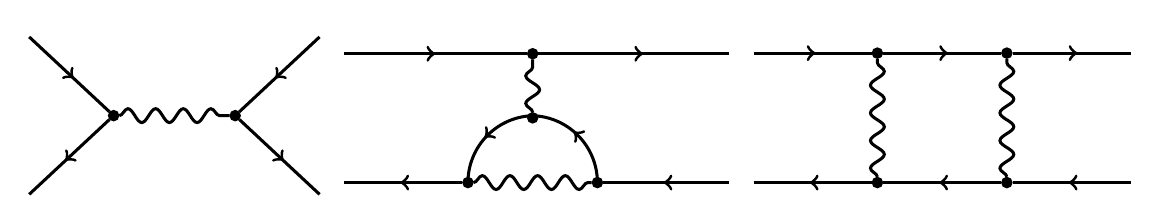
\begin{tikzpicture}[node distance=1cm and 1cm,line width=1.1pt]
  \coordinate[] (treei1);


  \coordinate[below=1 of treei1] (treei2);
  \coordinate[below=2 of treei1] (treei3);
  \coordinate[below=3 of treei1] (treei4);
  \coordinate[below=4 of treei1] (treei5);
  \coordinate[vertex,right=1 of treei3] (treev1);
  \coordinate[vertex,right=1.4 of treev1] (treev2);
  \coordinate[right=1 of treev2] (treev3);
  \coordinate[above=1 of treev3] (treeo1);
  \coordinate[below=1 of treev3] (treeo2);
  \draw[fermion] (treei2) -- (treev1);
  \draw[fermion] (treev1) -- (treei4);
  \draw[fermion] (treeo1) -- (treev2);
  \draw[fermion] (treev2) -- (treeo2);
  \draw[photon] (treev1) -- (treev2) node[midway,above=0.1] {};

  \coordinate[right=4 of treei4] (dummy1);
  \coordinate[above=0.15 of dummy1] (pengi1);

  \coordinate[vertex,right=1.5 of pengi1] (pengv1);
  \coordinate[vertex,right=1.5 of pengv1] (pengv2);
  \coordinate[right=0.75 of pengv1] (pengv3);
  \coordinate[vertex,above=0.75 of pengv3] (pengv4);
  \coordinate[vertex,above=0.67 of pengv4] (pengv5);
  \coordinate[left=2.32 of pengv5] (pengi2);
  \coordinate[right=2.42 of pengv5] (pengo2);
  \coordinate[right=1.6 of pengv2] (pengo1);
  \draw[antifermion] (pengv1) arc (180:90:0.85) ++(-1.1,1.0) node[left] {};
  \draw[fermion] (pengv2) arc (0:90:0.85) ++(-1.1,1.0) node[left] {};
  \draw[photon] (pengv1) -- (pengv2);
  \draw[photon] (pengv4) -- (pengv5);
  \draw[antifermion] (pengi1) -- (pengv1);
  \draw[antifermion] (pengv2) -- (pengo1);
  \draw[antifermion] (pengv5) -- (pengi2);
  \draw[fermion] (pengv5) -- (pengo2);

  \coordinate[right=5.2 of dummy1] (dummy2);
  \coordinate[above=0.15 of dummy2] (boxi1);
  \coordinate[vertex,right=1.5 of boxi1] (boxv1);
  \coordinate[vertex,above=1.5 of boxv1] (boxv2);
  \coordinate[vertex,right=1.5 of boxv1] (boxv3);
  \coordinate[vertex,right=1.5 of boxv2] (boxv4);
  \coordinate[left=1.5 of boxv2] (boxi2);
  \coordinate[right=1.5 of boxv3] (boxo1);
  \coordinate[right=1.5 of boxv4] (boxo2);
  \draw[antifermion] (boxi1) -- (boxv1);
  \draw[antifermion] (boxv1) -- (boxv3);
  \draw[antifermion] (boxv3) -- (boxo1);
  \draw[fermion] (boxv2) -- (boxv4);
  \draw[photon] (boxv1) -- (boxv2);
  \draw[photon] (boxv3) -- (boxv4);
  \draw[antifermion] (boxv2) -- (boxi2);
  \draw[fermion] (boxv4) -- (boxo2);

\end{tikzpicture}







\end{document}
